\documentclass[17pt]{beamer}
\usepackage[CJKspace]{xeCJK}
%\usepackage{newtxtext,newtxmath}	% use Times Roman font
%\usefonttheme{serif}
\usefonttheme{professionalfonts}
%\setbeamertemplate{theorems}[numbered]
\setbeamertemplate{caption}{\insertcaption} 	% no `Figure' prefix before caption

\mode<presentation> {

%\usetheme{default}
%\usetheme{AnnArbor}
%\usetheme{Antibes}
%\usetheme{Bergen}
%\usetheme{Berkeley}
%\usetheme{Berlin}
%\usetheme{Boadilla}
%\usetheme{CambridgeUS}
%\usetheme{Copenhagen}
%\usetheme{Darmstadt}
%\usetheme{Dresden}
%\usetheme{Frankfurt}
%\usetheme{Goettingen}
%\usetheme{Hannover}
%\usetheme{Ilmenau}
%\usetheme{JuanLesPins}
%\usetheme{Luebeck}
\usetheme{Madrid}
%\usetheme{Malmoe}
%\usetheme{Marburg}
%\usetheme{Montpellier}
%\usetheme{PaloAlto}
%\usetheme{Pittsburgh}
%\usetheme{Rochester}
%\usetheme{Singapore}
%\usetheme{Szeged}
%\usetheme{Warsaw}

%\usecolortheme{albatross}
%\usecolortheme{beaver}
%\usecolortheme{beetle}
%\usecolortheme{crane}
%\usecolortheme{dolphin}
%\usecolortheme{dove}
%\usecolortheme{fly}
%\usecolortheme{lily}
%\usecolortheme{orchid}
%\usecolortheme{rose}
%\usecolortheme{seagull}
%\usecolortheme{seahorse}
%\usecolortheme{whale}
%\usecolortheme{wolverine}

%\setbeamertemplate{footline} % To remove the footer line in all slides uncomment this line
%\setbeamertemplate{footline}[page number] % To replace the footer line in all slides with a simple slide count uncomment this line
\setbeamertemplate{navigation symbols}{} % To remove the navigation symbols from the bottom of all slides uncomment this line
}

%\setbeamertemplate{section page}
%{
%	\begingroup
%	\begin{beamercolorbox}[sep=12pt,center]{section title}
%		\usebeamerfont{section title}\insertsection\par
%	\end{beamercolorbox}
%	\endgroup
%}


\usepackage{graphicx} % Allows including images
\usepackage{verbatim} % comments
\usepackage{tikz-cd}  % commutative diagrams
\newcommand{\tikzmark}[1]{\tikz[overlay,remember picture] \node (#1) {};}
\usepackage{booktabs} % Allows the use of \toprule, \midrule and \bottomrule in tables
\usepackage{amssymb}  % \leftrightharpoons

\newcommand{\vect}[1]{\boldsymbol{#1}}
\newcommand*\sigmoid{\vcenter{\hbox{
\includegraphics{sigmoid.png}}}}

\makeatletter
\renewcommand{\boxed}[1]{\fbox{\m@th$\displaystyle\scalebox{0.9}{#1}$} \,}
\makeatother

%---------------------------- make slide margin narrower --------------------------------
%\newcommand\Wider[2][3em]{%
%	\makebox[\linewidth][c]{%
%		\begin{minipage}{\dimexpr\textwidth+#1\relax}
%			\raggedright#2
%		\end{minipage}%
%	}%
%}

%----------------------------------------------------------------------------------------
%	TITLE PAGE
%----------------------------------------------------------------------------------------

\title[China AGI group]{AGI 的一些基本概念} % The short title appears at the bottom of every slide, the full title is only on the title page

\author{YKY 甄景贤} % Your name
\institute[] % Your institution as it will appear on the bottom of every slide, may be shorthand to save space
{
Independent researcher, Hong Kong \\ % Your institution for the title page
\medskip
\textit{generic.intelligence@gmail.com} % Your email address
}
\date{\today} % Date, can be changed to a custom date

\begin{document}

\frame{\titlepage}

\begin{frame}
\frametitle{Talk summary}
\tableofcontents
\end{frame}

%---------------- this is for when you're using \part's ----------------------------------
%\begin{frame}
%\frametitle{Summary}
%
%{\usebeamerfont*{frametitle} Part I %\usebeamercolor[fg]{frametitle}
% ~ ~ ~ Deep reinforcement learning}
%%\tableofcontents[part=1]
%
%\vspace{1.5cm}
%{\usebeamerfont*{frametitle} Part II %\usebeamercolor[fg]{frametitle}
% ~ ~ ~ Logical structure}
%%\tableofcontents[part=2]
%\end{frame}

%----------------------------------------------------------------------------------------
%	PRESENTATION SLIDES
%----------------------------------------------------------------------------------------

%------------------------------------------------

%\part{title}

\section{什么是 归纳偏好? \\「没有免费午餐」}
\frame{\sectionpage}

\begin{frame}
\frametitle{机器学习 的 目的}
\begin{itemize}
	\item 机器学习 的 目的,是在某些「学习机器」的 \textbf{空间} 中,搜寻 符合要求的某些机器
	\item 例如在所有给定大小的神经网络中,搜寻符合 \textbf{目标函数} 的那些神经网络的 weights
\end{itemize}
\end{frame}

\begin{frame}
\frametitle{AI Winter}
\begin{itemize}
	\item 一般来说,AI 的 樽颈问题 就是 \textbf{搜寻空间} 太大,导致 学习 太慢
	\item 历史上「AI 寒冬」出现的原因,是因为 \textbf{基於逻辑} 的学习方法,导致 搜寻空间 的 组合数量爆炸,而没有很好的 heuristic(算法窍门)
\end{itemize}
\end{frame}

\begin{frame}
\frametitle{Inductive bias (归纳偏好)}
\begin{itemize}
	\item 每种学习方法都有它的 \textbf{归纳偏好}
	\item 换言之,在 搜寻空间 里预先 划分 某些部分 是不会搜索的
	\item 所以 偏好 令学习更快
	\item 但如果 偏好 太强,连 答案 所在的空间也删除了 \\
	``Throw the baby out with the water''
\end{itemize}
\end{frame}

\section{神经网络 的 力量 \\来自什么?}
\frame{\sectionpage}

\begin{frame}
\frametitle{神经网络的结构}
\begin{itemize}
	\item 一粒神经元 就是 一个 dot product 接著 一个 非线性函数:
	\begin{equation}
	\sigmoid \langle \vect{x}, \vect{w} \rangle
	\end{equation}	
	\item 这非线性函数 可以有很多种,例如:
	\begin{equation}
	\sigmoid (\xi) = \frac{1}{1 + e^{- \xi}}
	\end{equation}
\end{itemize}
\end{frame}

\begin{frame}
\frametitle{神经网络的结构}
\begin{itemize}
	\item 一层神经元 是 一个 矩阵 乘法:
	\begin{equation}
	\sigmoid( \; W \cdot \vect{x} \; )
	\end{equation}	
	\item 一个神经网络 是很多 层 的函数 composition $(f \circ f)$:
	\begin{equation}
	[ \sigmoid W ]^L \; \vect{x}
	\end{equation}	
\end{itemize}
\end{frame}

\begin{frame}
\frametitle{神经网络 的 特性}
\begin{itemize}
	\item 神经网络 是一个有很多 \textbf{参数} 的 函数
	\item 它是 \textbf{万能的 函数 近似器} [Cybenko 1989]
	\item 定理 的 证明 可追溯到 Weirstrauss 定理,即: 任意连续函数 可以用 多项式 近似
\end{itemize}
\end{frame}

\begin{frame}
\frametitle{神经网络 的威力来自「深度」}
\begin{itemize}
	\item 例如,假设 $\sigmoid$ 是 3次多项式
	\item 每增加一层 神经网络,等如
	\begin{equation}
	 (\mbox{多项式} \circ \mbox{多项式})
	\end{equation}
	\item 故,总体 的 多项式 次数 = $3^L$
	\item 换句话说 整体次数 呈 \textbf{指数式增长}
\end{itemize}
\end{frame}

\begin{frame}
\frametitle{神经网络 的威力来自「深度」}
\begin{itemize}
	\item \textbf{代数基本定理}:多项式 \textbf{次数} = 曲线 跨过 $x=0$ 多少次
	\begin{equation}
	\vcenter{\hbox{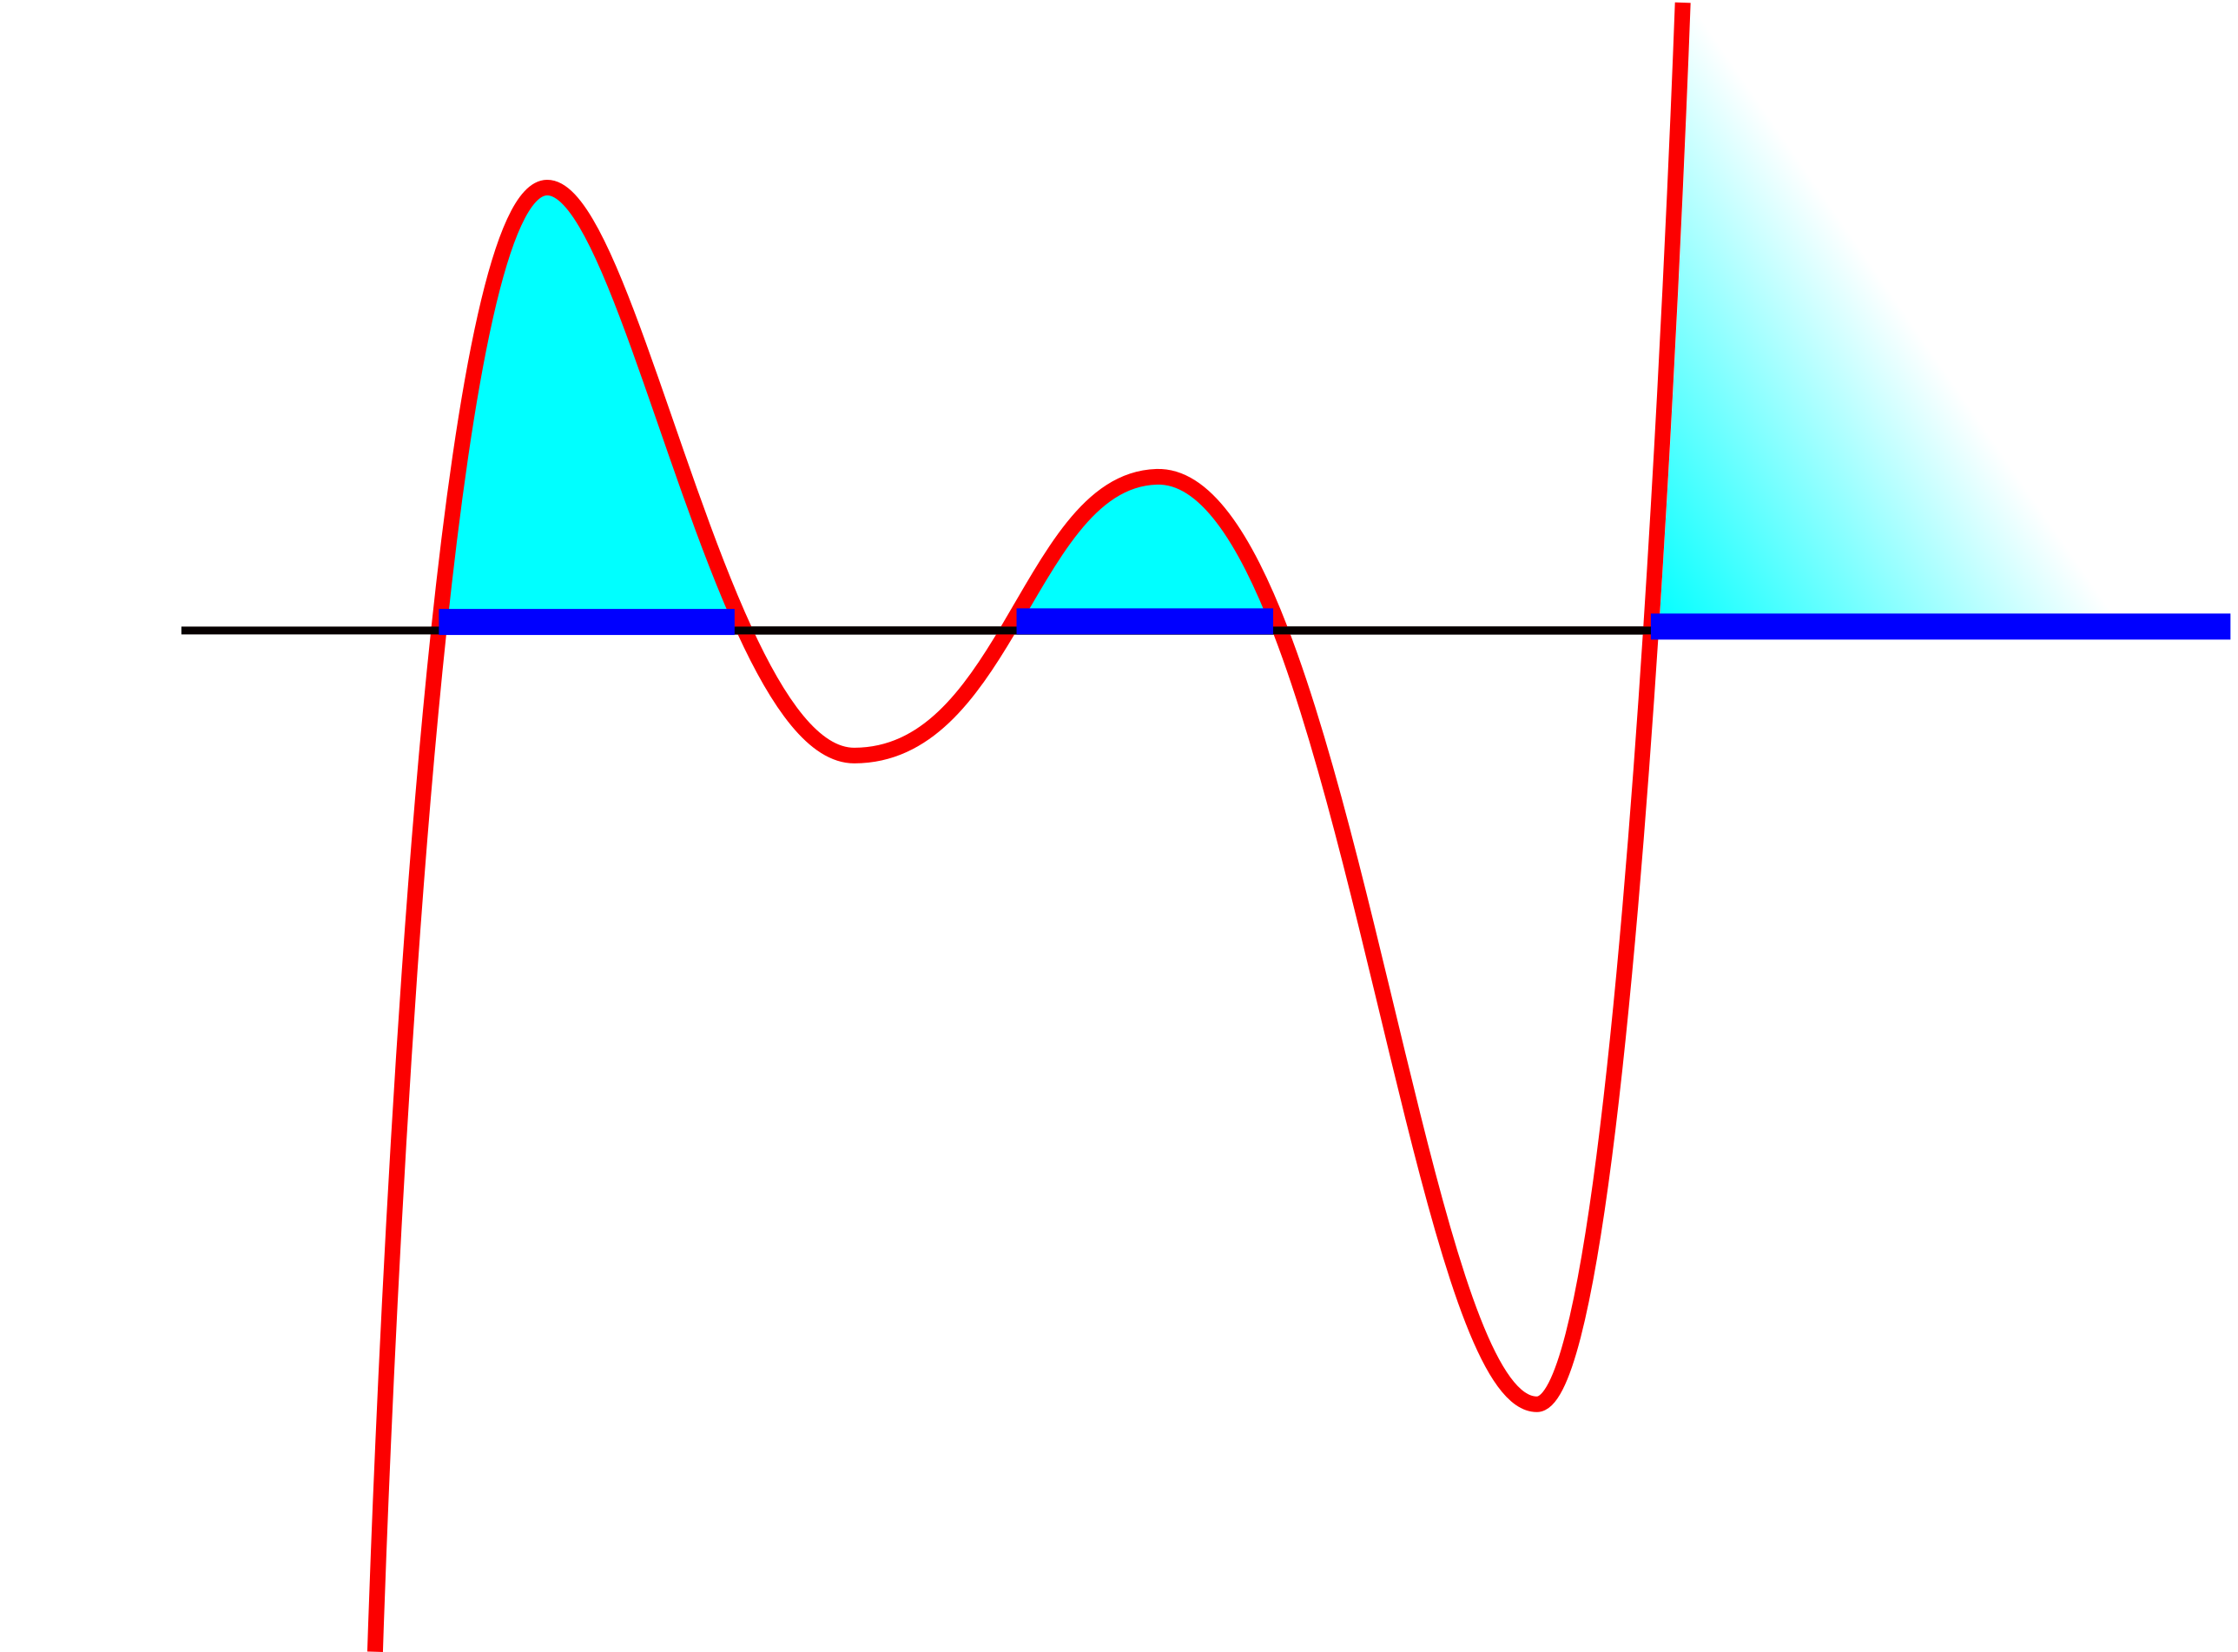
\includegraphics[scale=0.4]{../2018/zero-crossings.png}}}
	\end{equation}
	\item 高维: 曲面 对 分类空间 分割成 多少块
\end{itemize}
\end{frame}

\begin{frame}
\frametitle{神经网络 的威力来自「深度」}
\begin{itemize}
	\item 这和 VC-dimension 道理一样 [Vapnik–Chervonenkis 1971] 
	\item VC-dimension = 函数 能将 空间 分割成多少块
	\item 多层 神经网络 的 VC-dim 是 $O(N \log N)$ 其中 N  是 网络参数 的总个数,但证明用的是不连续的 阀函数
	\item 我估计 VC-dim 会是 指数增长的,但未有证明
\end{itemize}
\end{frame}

\begin{frame}
\frametitle{神经网络 的威力来自「深度」}
\begin{itemize}
	\item VC-dim \textbf{指数增长} 的意义,表示 神经网络 能 代表 一个 非常复杂的 \textbf{函数家族}
	\item 而 神经网络 的参数个数 相对地 很少,可以在 电脑上实现
\end{itemize}
\end{frame}

\begin{frame}
\frametitle{卷积 神经网络 的 启示}
\begin{itemize}
	\item Yann LeCun 在 1989 发明了 ConvNet,彻底改革了 机器视觉领域,最近得了 Turing 奖
	\begin{equation}
	\nonumber
	\vcenter{\hbox{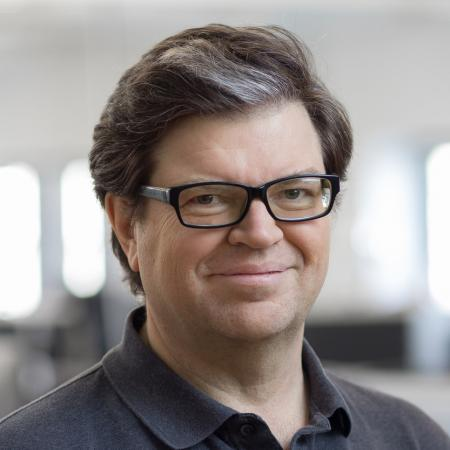
\includegraphics[scale=0.25]{Yann-LeCun.jpg}}}
	\end{equation}
\end{itemize}
\end{frame}

\begin{frame}
\frametitle{卷积 神经网络 的 启示}
\begin{itemize}
	\item CNN 将普通 NN 的 点积 用 卷积 代替:
	\begin{equation}
	\boxed{\mbox{点积}} \quad \sigmoid \langle \vect{x}, \vect{w} \rangle \rightsquigarrow \sigmoid( f * g ) \quad \boxed{\mbox{卷积}}
	\end{equation}
	\item 而 卷积 具有 \textbf{平移 不变性},有利於 视觉:
	\begin{equation}
	T_x(f) * g = T_x( f * g )
	\end{equation}
	\item 这是一种 \textbf{归纳偏好},令 学习 更快
\end{itemize}
\end{frame}

\begin{frame}
\frametitle{卷积 神经网络 的 启示}
\begin{itemize}
	\item 其实 \textbf{视觉} 需要的是 \textbf{仿射} (affine) 不变性,它包括 平移、旋转、放大缩小 等
	\item 但 似乎 单单是 平移不变性 所带来的 \textbf{学习加速},已足以令 CNN 在 2012 年超越了人类水平
	\item 可见,\textbf{归纳偏好} 在 深度学习 里 仍然是很有用的
\end{itemize}
\end{frame}

\section{Turing 机 与 逻辑 的 宇宙性}
\frame{\sectionpage}

\begin{frame}
\frametitle{有限自动机}
\begin{itemize}
	\item 通常用一个 tuple 定义(从略):
	
\end{itemize}
\end{frame}

\begin{frame}
\frametitle{The problem with predicate logic}
\begin{equation}
\forall x,y,z. \; \mbox{father}(x,y) \wedge \mbox{father}(y,z) \rightarrow \mbox{grandfather}(x,z)
\end{equation}
\begin{itemize}
	\item This involves \textbf{variable substitutions} which are troublesome to handle with neural networks. \\
	(The difficulty seems to come from the cylindric-algebraic structure of predicate logic:  if a formula have variables $x_1, x_2, x_3, ...$, we would need to consider the domain $D \times D \times D \times ...$ where $D \ni x_i$)
\end{itemize}
\end{frame}

\section{经典逻辑 AI 系统 的 基本结构}

%\subsection{Plan A: co-operative co-evolution (COCO)}

%\subsection{Plan B: hybrid neural + graph}

%\subsection{Plan C: geometric models}

%\subsection{Plan D: ``quantum'' Hilbert-space operators}

\begin{frame}
\frametitle{Relation algebra}
Given that:
\begin{equation}
\mbox{Father} \circ \mbox{Father} = \mbox{Grandfather}
\end{equation}
we can deduce:
\begin{eqnarray}
\mbox{john Father paul} \\
\mbox{paul Father pete} \\
\Rightarrow \mbox{john Father $\circ$ Father pete} \\
\Rightarrow \mbox{john Grandfather pete}
\end{eqnarray}
via \textit{direct} substitution of equal terms.
\begin{itemize}
	\item  Relation algebra appears very \textit{natural} and similar to human thinking
\end{itemize}
\end{frame}


%\cite{Jacobs1999}

\begin{comment}

\begin{frame}
\frametitle{References}
\footnotesize{
\begin{thebibliography}{99} % Beamer does not support BibTeX so references must be inserted manually as below
\bibitem[]{} Bart Jacobs (1999)
\newblock Categorical logic and type theory
% \newblock \emph{North Holland, Studies in logic} v141.

\bibitem[]{} Robert Goldblatt (2006)
\newblock Topoi -- the categorical analysis of logic

\end{thebibliography}
}
\end{frame}
\end{comment}

\begin{frame}
We're looking for developers to implement a prototype.

\vspace*{1cm}
\Large{\centerline{Thank you}}

%\vspace*{1cm}
%\Large{\centerline{The End}}
\end{frame}

\end{document} 